\chapter{System Implementation}

This chapter describes how the system is actually being implemented.

\section{Go language interfaces}

The Go programming language provides a powerful feature called interfaces. An interface is a collection of method signatures that a type, like a struct, can implement. Interfaces allow to define a set of methods that a type must implement to be considered an instance of that interface. This allows to write code that is more flexible, especially for testing purposes.

We setup each one of the checks as a separate interface, so that we can easily test them in isolation and also to make it easier to manage the codebase and add new checks in the future, like if they are modules that can be added or removed from the system.

The modularity of a project is a key feature that allows one to easily extend the codebase and add new features. Without modularity, the codebase would be a monolithic block of code that is difficult to handle with the time and the natural growth of a codebase.

Therefore, we created different packages for the different categories of modules, like \textit{check} and \textit{version} plus some utility packages like \textit{parsing}, \textit{output} and \textit{mapping}.

The scopes for the different packages are the following:

\begin{itemize}
  \item \textit{check}: it aggregates the different controls on a property of the device, like the \textit{Check correct time} or the \textit{Check VNC credentials};
  \item \textit{version}: contains the modules to determine whether the software running on the device is up-to-date or not;
  \item \textit{parsing}: it handles the parsing of the input parameters, for example the verbose flag or the list of checks to run;
  \item \textit{output}: it manages the output of the checks, like the output format and the output file;
  \item \textit{mapping}: contains the effective available mapping for the tool.
  \item \textit{variab} and \textit{utils}: are utility packages that contain some common structures and functions that are used across the codebase.
\end{itemize}

The structure of a module is composed of the actual interface, named as \textit{<module>Interface}, where \textit{<module>} is the name of the module, a struct that implements the interface, named as \textit{<module>Struct} and a function that returns an instance of the struct, named as \textit{new<Module>}.
All the fields of the struct are private, and the public method is the one that returns the method of the interface.

A practical example is the \textit{CheckTime} module, which checks if the time of the device is correct. The interface is defined as follows:

\begin{lstlisting}[style=golang]
type checkTimeInterface interface {
	checkTime(context.Context) variab.Result
	getNtpHmiConfig(context.Context) (*hmiDateTimeDto, error)
	getRealTimeWrapper() (*time.Time, error)
}
\end{lstlisting}

The structure is defined as follows:

\begin{lstlisting}[style=golang]
type checkTimeStruct struct {
	delta             time.Duration
	getCliTime        func() (*string, error)
	getRealTime       func(string, string, string, time.Duration) (*time.Time, error)
	[omitted]
	timeout           time.Duration
}
\end{lstlisting}

There is an instance of the struct that is returned by the function \textit{newCheckTime}:

\begin{lstlisting}[style=golang]
func newCheckTime() checkTimeInterface {
	return &checkTimeStruct{
		delta:          DELTA_DURATION,
		getCliTime:     getCliTime,
		getRealTime:    getRealTime,
		[omitted]
		timeout:        utils.TIMEOUT,
	}
}
\end{lstlisting}

and the public method is the one that returns the method of the interface:

\begin{lstlisting}[style=golang]
var checkTime checkTimeInterface = newCheckTime()

func CheckTime(ctx context.Context) variab.Result {
	return checkTime.checkTime(ctx)
}
\end{lstlisting}

% Some of the variables are omitted for brevity. The other ones come from both some constants and some utility variables defined across the codebase. 
The interface has a method that checks if the time of the device is correct, and it always returns a \textit{variab.Result} struct that contains the result of the check.

The \textit{Result} structure of the package \textit{variab} is a common structure that is used to return the result of the checks. It contains a concise message for the output, an optional recommendation to solve the issue, a severity level ranging from \textit{none} to \textit{high} and an operation status, where \textit{OK} means that the module completed the task without noticing any vulnerability, \textit{ISSUE} means that the module contains a potential weakness, \textit{EXECUTION\_ERROR} in the case of an unhandled exception, \textit{UNKNOWN} otherwise. This structure is used by all the modules to return the result of a module. Any exception is handled in order to guarantee the robustness of the tool in case of any failure, allowing the user to always obtain a valid output.

\begin{lstlisting}[style=json, caption={Result struct}]
{
  "message": string,
  "recommendation": string,
  "severity": none|low|moderate|high,
  "status": OK|ISSUE|EXECUTION_ERROR|UNKNOWN
}
\end{lstlisting}

This composition is common to all the modules, and it allows us to easily test the modules in isolation, by mocking the dependencies of the struct. This is done by creating a new struct that implements the same interface, but with mocked methods, and then injecting this struct in the test. This way, we can test the module without having to actually run the code that is being mocked. This is a powerful feature of the Go language that allows to write more robust and maintainable code. More to follow about the testing phase in the next chapter.

\section{First sprint}

The first sprint has the goal of implementing the first set of modules, as expressed in the sprint planning. We are going to detail the implementation of every story from the sprint backlog.

\subsection{CheckTime module}

The \textit{CheckTime} module checks if the datetime of the device is correct. This is a fundamental thing to verify because the issues with the devices not connecting to the internet and to the cloud are most of the time due to the incorrect datetime, leading to an error with the SSL certificate. In fact, if the date is not correct, the SSL certificate could result as expired or not yet valid, warning the user that the connection is not secure.

It does so by getting the time from the device and the real-time from a remote server, and then comparing the two times. If the difference between the two times is greater than a certain threshold, expressed in a range of few minutes, then the module returns an \textit{ISSUE} status, otherwise it returns an \textit{OK} status. Of course, this module works with an active internet connection only; if the device is not connected to the internet, then the module returns a valid execution error.

To perform the execution, it runs the following steps:
\begin{itemize}
  \item first, it gets the UNIX timestamp, an integer number representing the elapsed seconds since 1\textsuperscript{st} January 1970, by executing the command \texttt{date +\%s} on the local shell;
  \item then it calls a remote endpoint that returns the real datetime;
  \item it parses the two datetimes;
  \item finally, it compares their difference and returns the result.
\end{itemize}

If any of the steps fails, the module returns the execution error status.

% proxy network call qui?

\subsection{JSON output}
\label{sec:json-output}

Every module returns a structure representing the result of the execution, a brief message and a recommendation to solve the potential issue. The modules runner collects all the results from the modules in a \textit{Report} type variable, that is defined as a map of maps, in order to have the direct mapping of the result of the module under the category and the name of the module.

The resulting type is therefore given to the \textit{output} package, which is responsible for the desired destination format. The default formatter is JSON, but it can be easily extended to support other formats like YAML by importing or implementing the corresponding marshaler, that is a function that transforms the encoding of an \textit{any} value to the desired format.

By default, the output is printed to the standard output of the terminal, but the destination can be redirected to a file by using the built-in method with the \texttt{-d} flag.

The output can be printed in a pretty format by using the \texttt{--pretty} flag, useful for human readability. Anyway, the predefined formatting is minified. The formatter can be chosen by using the \texttt{-o} flag, followed by the desired format. For example, to output the result in YAML format in the terminal the command is \texttt{./scantool scan -o yaml}, or \texttt{./scantool scan -o yaml -d output.yaml} to redirect the output to a file.

The list of the active modules is available with the command \texttt{./scantool list}, printed in the standard output of the terminal, one for line.

For example, given the execution of the datetime module only, issued with the command \texttt{./scantool scan --list "check.time" --pretty} with no further parameters, the output structure would be as the following:

\begin{lstlisting}[style=json, caption={Output of the datetime module}]
{
"check": {
  "time": {
    "message": "The current datetime is synced",
    "recommendation": "No action required",
    "severity": "none",
    "status": "OK"
  }
}
\end{lstlisting}

\subsection{Cross build script}

The Go programming language provides a powerful feature called cross-compilation. This allows to build the binary for a different architecture than the one of the machine that is building it. This is useful to build the binary for a different architecture, like ARM, that is the architecture of some of the devices that we are going to use for debugging purposes.

Go provides the built-in command \texttt{go build <file>} that builds the binary for the current architecture, but it also provides the \texttt{GOOS} and \texttt{GOARCH} environment variables that can be set to the desired values to build the binary for a different architecture.

The former is the operating system, and the latter is the architecture. Possible values useful for the project are \texttt{linux} for the operating system and \textit{arm}, \textit{arm64} and \textit{amd64} for the architecture. All the available values can be found in the official documentation of the Go programming language.~\cite{go-valid-goos-goarch-combinations}

By default, the binary includes debug symbols, that are useful for debugging purposes, but they are not necessary for the production environment. They increase the size of the binary to several megabytes, and they are not needed by the end user. In particular, we add two flags to the build command:~\cite{go-ldflags-all,go-ldflags-s-w}
\begin{itemize}
  \item \texttt{-s} turns off generation of the Go symbol table;
  \item \texttt{-w} turns off debugging information, not being able to trace the resulting binary with the \texttt{gdb} debugger.
\end{itemize}

In the context of the automatic pipeline that builds the binary for the different architectures, we also inject the version number of the binary in the build command, by using the \texttt{-X importpath.name=value} flag. This flag allows to set the value of the string variable in \textit{importpath} named \textit{name} to \textit{value}.~\cite{go-ldflags-all}

Furthermore, we also explicitly set the environment variable \texttt{CGO\_ENABLED=0} to disable the use of the machine C compiler. Anyway, that is disabled by default when cross-compiling and the go builder chooses the appropriate compiler for the target architecture.~\cite{go-cgo-compiler}

Finally, we set the \texttt{-trimpath} flag to remove the absolute path of the source files from the binary, in order to make the binary reproducible. This is a good practice to follow, as it does not leak any information about the source code and the environment where the binary was built.~\cite{go-trimpath-arg}

The resulting binary for each architecture is placed in a tree of directory, where the root directory is the version of the binary, and the subdirectories are the architectures. The filename of the binary is the same as the name of the project, that is \texttt{scantool}.

The final build command is the following:
\begin{lstlisting}[caption={Go tool cross-build command}]
  env GOOS=$GOOS GOARCH=$GOARCH CGO_ENABLED=0 go build -trimpath -ldflags="-s -w -X 'main.VERSION=$version'" -o $output_base_dir/$version/$arch/$filename main.go
\end{lstlisting}

The difference between the size of a build without any optimization and an optimized build is quite relevant. Taking as example the architecture \textit{arm64} on the \textit{Linux} operating system, the former takes 12MB and the latter takes 7.7MB. On industrial devices, such size difference matters a lot in terms of storage and bandwidth to download it on the fly when needed.

\subsection{Scan OS version}

The custom board of the industrial devices powers a custom Linux distribution, that is based on the Yocto Project. The updates are managed by the internal department of the company, with an internal version manager. The updates are not automatic, and they have to be requested by the customer.

This module monitors whether the operating system is at its latest version or not. Given that the estimated work to implement it as a single block is not trivial, we can split it into two different specializations: the first one is the one that checks the version of the operating system by retrieving the build date, and the second one is the one that checks the version of the operating system by reading the online repository.

The Device Settings API, a set of endpoints used to retrieve the information about the status of the device and to potentially change them, provides among other things the version number and the build date of the operating system. There is the \texttt{/api/v1/management/mainos} endpoint that returns a JSON object structured as follows:

\begin{lstlisting}
{
  "version": "4.2.323",
  "date": "2024-04-17T06:00:00.000Z"
}
\end{lstlisting}

The module is implemented by the \textit{versionOsInterface} and \textit{versionOsStruct} structure. The interface is defined as:

\begin{lstlisting}[style=golang]
type versionOsInterface interface {
  getOsInfo(context.Context) (*versionOsApiDto, error)
  checkOsVersion(context.Context) variab.Result
}
\end{lstlisting}

and the structure is formed of the following fields:

\begin{lstlisting}[style=golang]
type versionOsStruct struct {
  xMonthAgo      int
  [omitted]
}
\end{lstlisting}

The \textit{xMonthAgo} field is the threshold expressed in a range of few months. The \textit{getOsInfo} method retrieves the information about the operating system from the Device Settings API, and the \textit{checkOsVersion} method actually performs the comparison.

\subsubsection{Offline date based}

The first specialization of the module checks the version of the operating system by reading the build date of the system. This is done by retrieving the build date of the system from the Device Settings API, that is the \textit{date} field of the API response. The date is then compared with the current date, and if the difference is greater than a certain threshold then the module returns an issue, otherwise it returns an OK status throug the \textit{Result} structure.

\subsubsection{Online version based}

This specialization should compare the local version of the operating system with the latest version available somewhere online. Since the company does not provide a public repository for the updates, this module cannot be implemented yet. The idea is to have a list of the latest versions for the different device models and to compare the local version with the latest one. If the local version is not updated, then the module returns an issue, otherwise it returns an OK status. This is a future work that can be implemented when the company will start to provide a public repository for the updates. As a matter of fact, this story has been suspended in the context of our project.

\subsection{Default BSP credentials}

Setting common passwords is a bad practice, as they let an attacker to potentially gain unauthorized access to the management of the device.

The devices ship with some default credentials for the two users that are available on the system, named \textit{admin} and \textit{user}. The credentials are required to interact with the Device Settings.
% They are asked to be changed at the first login, but the user could skip the step and keep the default ones.\footnote{verify}

The module checks whether the default credentials are still in use by trying to login with a pre-defined set of passwords for the two users. The module performs $2*|harcodedPasswords|$ HEAD requests to an arbitrary endpoint of the Device Settings API and it checks the status code of the response. If one of the responses' status codes is \textit{200 Success}, meaning that the authorization has been granted and therefore username and password match, then the module returns an issue with a high severity, otherwise it returns an OK status.

This security control is possible without stumbling into the device's built-in authentication rate-limiting because the total number of requests is below the threshold of the requests for minute that the device accepts before temporarily blocking the access from that access.

The module is implemented by the \textit{checkCredentialsSystemSettingsInterface} and \textit{checkCredentialsSystemSettingsStruct} structure. The interface is defined as:

\begin{lstlisting}[style=golang]
type checkCredentialsSystemSettingsInterface interface {
	checkCredentialsSystemSettings(context.Context) variab.Result
}
\end{lstlisting}

and the structure is made of the following fields:

\begin{lstlisting}[style=golang]
type checkCredentialsSystemSettingsStruct struct {
  [omitted]
  hmiHeadRequest func(string, time.Duration, *string, *string) (*http.Response,error)
  users          []string
  passwords      []string
}
\end{lstlisting}

The \textit{hmiHeadRequest} function is a utility function that performs a HEAD request to the given URL with a certain user and password. The \textit{users} and \textit{passwords} fields are the list of users and passwords to try to login with.

\subsection{Scan SSH port}

The SSH protocol, which stands for \textit{Secure Shell}, is a cryptographic network protocol that allows to securely connect to a remote device. It is widely used in the industry to connect to the devices for the purposes of debugging, maintenance and monitoring. The SSH protocol is based on the client-server model, where the client connects to the server and authenticates itself by providing a username and a password or a public key. The server then verifies the credentials and grants access to the client if they are correct.

The SSH protocol is based on the TCP protocol, and it uses port 22 by default. The server, that is the industrial device, listens on port 22 for incoming connections. Because of the widespread adoption of the SSH protocol, that port is a common target for attackers who try to gain unauthorized access to the devices.

This story is a specialization of a wider set of stories that check the status of the different services running on the device. The idea is to check whether the status of the service reported by the Device Settings API matches with the actual status of the service, and if enabled to warn that a port is exposed and therefore to be informed about the potential risks.

The module is implemented by the \textit{checkServicesInterface} and \textit{checkServicesStruct} structure. The interface is defined as:

\begin{lstlisting}[style=golang]
type checkServicesInterface interface {
  checkServices(context.Context, string) variab.Result
  hmiConfig() (*hmiServicesDto, error)
}
\end{lstlisting}

and the structure is composed of the following fields:

\begin{lstlisting}[style=golang]
type checkServicesStruct struct {
  isPortOpen     func(uint, time.Duration) (bool, error)
  [omitted]
}
\end{lstlisting}

The \textit{hmiConfig} function retrieves the information about the services from the Device Settings API, and the \textit{checkServices} function actually performs the check. The API endpoint is located at \texttt{/api/v1/services} and it returns a JSON object structured as a list of objects for each service, where each object contains its id, the name and the status.

The \textit{isPortOpen} function is a utility function that checks if the port is open on the device. It works by trying to open a socket on the port defined by a predefined map that contains a list of default ports for each of the services. Depending on the protocol, the function tries to connect to each of the ports and returns true if the connection is successful, otherwise it returns false.

By combining the two functions, the module checks if the SSH port status reported by the Device Settings API matches the actual status of the port.

\subsection{Check VNC credentials}

As part of the services that are running on the device, one of them is the VNC service. VNC, which stands for \textit{Virtual Network Computing}, is a cross-platform graphical desktop sharing system to remotely control another computer. It transmits the screen of the remote device to the client, and it allows to interact with it by sending the mouse and keyboard events. It uses the RFB - \textit{Remote Framebuffer} - protocol that governs the format of the data that passes between the client and server within the VNC system. The protocol itself does not require a mandatory authentication method, but is supports many of them, like a password or a certificate.

If the service is not properly configured and does not require a password to connect, then an attacker could potentially gain unauthorized direct access to the graphical interface and perform any operation that a legitimate user could do.

The module checks whether the VNC service is configured with a password or not. It does so by retrieving the configuration, in particular the port on which the service is running, from the Device Settings API, and then implementing the protocol itself to get the required authentication method. If the authentication method is not set, then the module returns an issue with a high severity, otherwise it returns an OK status.

\subsubsection{RFB protocol}

The RFB protocol is defined in the RFC 6143~\cite{rfc6143}. It works using the TCP protocol for the transport layer. The server, that is the industrial device, listens on the default port 5900 or on a custom one defined by the customer in the Device Settings.

The protocol expects the following steps:

\begin{enumerate}
  \item the client connect to the server and the server sends the protocol version; the \textit{ProtocolVersion} message consists of 12 bytes interpreted as a string of ASCII characters in the format \texttt{RFB xxx.yyy\textbackslash n} where \texttt{xxx} and \texttt{yyy} are the major and minor version numbers, left-padded with zeros: the only published protocol versions at this time are 3.3, 3.7, and 3.8. Other version numbers are reported by some servers and clients, but should be interpreted as 3.3 since they do not implement the different handshake in 3.7 or 3.8.
  \item the client replies to the server agreeing with its supported version, which must be less or equal to the one of the server;
        \begin{itemize}
          \item if the version is 3.3, then the server directly replies with a single integer number representing the security type;
          \item otherwise, the server replies with a list of numbers representing the security types that the server supports;
        \end{itemize}
  \item at this point, instead of proceeding with the protocol, we close the connection and we return the security type.
\end{enumerate}

If the security type is equal to the number 1, the server does not require any authentication. If the number is equal to 0, this is not expected and probably something went wrong in the implementation of the protocol. Both cases return as result a high severity issue. \\
If the security type is greater or equal to number 2, then the server correctly requires some access control. Note that we said greater than two and not strictly equal to 2 because other security types exist but are not publicly documented.

\begin{figure}[ht]
  \centering
  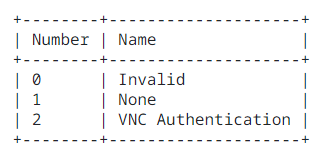
\includegraphics[width=0.5\textwidth]{chapters/05/assets/rfc6143-security-types}
  \caption{RFC 6143 security types}
  \label{fig:rfc6143-security-types}
\end{figure}

The module is implemented by the \textit{checkVncCredentialsInterface} and \textit{checkVncCredentialsStruct} structure. The interface is defined as:

\begin{lstlisting}[style=golang]
type checkCredentialsVNCInterface interface {
	checkCredentialsVNC(context.Context) variab.Result
}
\end{lstlisting}

and the structure contains the following fields:

\begin{lstlisting}[style=golang]
type checkCredentialsVNCStruct struct {
  [omitted]
  vncConn               func(string, time.Duration) (bool, net.Conn)
  vncProtocolVersion    func(net.Conn) ([]byte, error)
  vncAuthType3          func(net.Conn) (uint32, error)
  vncAuthType7_8        func(net.Conn) (uint32, error)
}
\end{lstlisting}

The \textit{vncConn} function creates the connection to the VNC server, the \textit{vncProtocolVersion} function retrieves the protocol version, the \textit{vncAuthType3} function retrieves the authentication method for version 3 of the protocol, and the \textit{vncAuthType7\_8} function retrieves the authentication method for the versions 7 and 8 of the protocol.

The \textit{checkCredentialsVNC} function performs the check by combining the functions above.

\subsection{Check certificate expiration}

The device uses the HTTPS protocol to expose the Device Settings UI and API and the optional web page of the running project. The HTTPS protocol is a secure version of the HTTP protocol that uses the SSL/TLS protocol to encrypt the data that passes between the client and the server. The SSL/TLS protocol uses a certificate to establish the identity of the server and to encrypt the data that passes between the client and the server. This behaviour is needed to prevent an attacker from intercepting the data that passes between the client and the server.

The certificate is issued by the company authority and it is valid for a certain period of time, usually years. A customer can upload a custom certificate to the device. The certificate is stored in the device.

The module checks whether the certificate is expired or not. Go provides built-in packages called \texttt{encoding/pem} and \texttt{crypto/x509} that allow to parse the certificate and to extract the expiration date. The former implements the PEM data encoding, which originated in \textit{Privacy Enhanced Mail}. The most common use of PEM encoding today is in TLS keys and certificates~\cite{go-package-pem}. The latter allows parsing and generating certificates, certificate signing requests, certificate revocation lists, and encoded public and private keys. It also provides a certificate verifier with a chain builder~\cite{go-package-x509}.

In particular, the certificate is read as bytes from the file system, then it is parsed by the \texttt{pem.Decode} function that returns a \texttt{pem.Block} structure. The \texttt{Block} structure contains the type of the block and the bytes of the block. The bytes are then passed to the \texttt{x509.ParseCertificate} function that returns a \texttt{x509.Certificate} structure. The \texttt{Certificate} structure also contains the expiration date of the certificate.

The expiration date is then compared with the current date: if the expiration date happens in less than 30 days, the module returns an issue. If the valid days left are less than 30, the severity is low; if they are less than 15, the severity is moderate; if they are less than 1, the severity is high.
-
The implementation of the module is defined by the \textit{checkCertificatesInterface} and \textit{checkCertificatesStruct} structure. The interface looks like:

\begin{lstlisting}[style=golang]
type checkCerticatesInterface interface {
	checkCertificates(context.Context) variab.Result
}
\end{lstlisting}

and the structure is made up of the following fields:

\begin{lstlisting}[style=golang]
type checkCertificatesStruct struct {
	hmiCertPath string
	loadCertFile func(string) ([]byte, error)
}
\end{lstlisting}

The \textit{hmiCertPath} field is the path to the certificate file, and the \textit{loadCertFile} function reads the certificate file from the file system. The \textit{checkCertificates} function performs the check by combining the functions above.

\subsection{Verbose flag}

This flag is a common one that is used in the command line interface of the tool to increase the verbosity of the output. By default, the output is minimal and it contains only the result of the checks, but by using the \texttt{--verbose} flag the output is increased to include more information about the execution of the modules.

The flag is implemented by taking advantage of the hooks provided by \textit{spf13/cobra}, that is the package that we use to implement the command line interface. The \texttt{cobra.Command} structure provides a \texttt{PersistentPreRun} callback that is called before the execution. We use this callback to set the verbosity level of the output for the \textit{zerolog} package with the \texttt{zerolog.SetGlobalLevel} function.

This flag is defined as persistent, meaning that it is available for every command and subcommand and it is only defined once.

\subsection{Add YAML report formatter}

In addition to the JSON output, we also add the YAML output format. The YAML format is a human-readable data serialization standard that can be used in conjunction with all programming languages and is often used to write configuration files. The YAML format is more human-readable than the JSON format. It is not native in the Go programming language, but there is an official porting available at the \texttt{gopkg.in/yaml.v3} package.

As described in~\cref{sec:json-output}, the output package is responsible for the output of the results in the desired format. The default format is JSON, but it can be easily extended to support other formats like YAML by importing the corresponding marshaler.

In this case, we add the \texttt{yaml.Marshal} function to the output package the \textit{Report} structure. If the user specifies the \texttt{-o yaml} flag, then the output is formatted in YAML to the desired destination.

The high modularity of the Go language and of the project allows to easily extend the output formats by simply adding few lines of code. This is a powerful feature of the Go language that allows to write more maintainable code.

\section{First sprint retrospective}

The first sprint has been completed successfully. All the expected modules but one have been implemented. For each of the tests, we have written comprehensive unit tests that run on demand. The implementation of the modules has been straightforward. The use of the interfaces has allowed to easily test the modules in isolation, by mocking the dependencies of the struct.

The only module that has not been implemented is the one that checks the version of the operating system by reading the online repository. This is because the company does not provide a public repository for the updates, and therefore we cannot implement the module yet. This is a future work that can be implemented when the company will provide a public repository for the updates.

Given that the first sprint has been completed successfully, we can move on to the second sprint. We did a meeting to show the results of the sprint to the office and to discuss the next steps. The feedback has been positive, and the team is happy with the results. The next sprint focuses on the implementation of more server side utilities and some more modules.

\section{Second sprint}

The second sprint has the goal of implementing the following set of modules:

\begin{itemize}
  \item Create cloud web app
  \item Implement proxy network call
  \item Automatic build and deployment
  \item Enable to download latest version of the tool
  \item Support internationalization
\end{itemize}

These are new features useful for the future adoption of the tool in the company.

The first two are server side utilities that are needed to prepare the infrastructure for future development of the tool in terms of strictly network policies and user billing. In fact, the company is interested in the possibility to offer the tool as a service to the customers, and therefore it is necessary to have a server side application in order to handle the functioning. Furthermore, as previously said, industrial network policies are very strict and usually they do not allow to connect directly to the internet, and therefore a proxy is needed to perform the network calls. \\
For example, given the case of a version check, if the remote location on which the version is stored happens on a third-party endpoint, like for an external dependency, each network administrator for each customer should manually allow the connection to that location, and beforehand the company should provide the list of the locations to allow and keep it updated. In order to avoid this, the company can provide a proxy server that is the only one that connects to the internet. The tool can then connect to the proxy server. This way, network administrators only have to allow the connection to the proxy server, that is already expected for the standard operation of the device.

The second and third points are about the automatic build and deployment of the tool. The company is interested in the possibility to automatically build the tool for the different architectures and to deploy it on the devices. This is also useful for testing purposes, as the build is preceded by the execution of the tests and also for the continuous integration and continuous deployment of the tool.

The latest point aims to provide internationalization, that is the support for different languages. The company is interested in the possibility to offer the tool in different languages, in order to make it more accessible to customers.

\subsection{Create cloud web app}

Recalling~\cref{sec:platform-applications}, the cloud app is an entire runtime made by a frontend and a backend that is visible through the platform website. The frontend is a VueJS application and the backend uses NestJS as the framework for handling the controllers, the models and the logic. Both the frontend and the backend are written in TypeScript and both implement the authentication with the platform, as it is really integrated with the platform itself and cannot be used in a standalone mode.

The skeleton of the application is generated by a public utility developed by the company, which is available on the public NPM registry. This utility generates the boilerplate code for the frontend and the backend, with many features already implemented, like the authentication with the platform, basic routing, controllers and models needed to complete the first installation on the platform.

The app also provides a running configuration of \textit{PostgreSQL} database that is used to store its data. The database is also deployed on the Kubernetes cluster.

The application has to be deployed on a Kubernetes cluster. The code also contains the required chart files, customized for the application, that are used by the Helm package manager to deploy the application on the cluster, and the Dockerfile that is used to build the Docker image of the application.

Once the deployment is live on the cluster, the application can be linked to the platform store by using the public REST API of the platform. Doing so, the application is visible on the platform website and it can be accessed by the customers.

\subsection{Implement proxy network call}

As said, usually the industrial networks attached to the devices are very strict and do not allow to communicate with every host on the internet. This is a security measure that is taken to reduce the risks of exposing relatively weak devices. In fact, according to internal statistics, unfortunately the devices are usually not updated frequently by the customers and they are not patched for the latest vulnerabilities. The goal of the tool described in this thesis is also to make aware the customers of a potential vulnerability that could be exploited by an attacker and new available updates. In order to do so, the tool has to communicate with the internet to check the latest version of the software. How to do that given all the constraints?

The solution we thought is to provide a proxy server that is the only one that connects to the final endpoints. The tool can then connect to the proxy server. This way, network administrators only have to allow the connection to the proxy server, that is already expected for the standard operation of the device.

The proxy server is managed by a controller on the cloud app backend. The controller is responsible for handling the incoming requests from the tool and for forwarding them to the respective methods. The controller is also responsible for handling the authentication with the platform. It is written in TypeScript and it uses the NestJS framework.

The proxy controller is a class that is decorated with the \texttt{@Controller} decorator, that is provided by the NestJS framework, with the parameter that is the base path of the controller. All the requests starting with that path are handled by the controller. A decorator is a special declaration that can be attached to a class, method or property, and it is used to modify their behaviour. The class is also decorated with \texttt{@ApiTags}, needed to generate the OpenAPI documentation, and by a \texttt{@UseInterceptors} directive with the \textit{LoggingInterceptor} custom one that logs the incoming requests. \\
The class contains the declaration of the services that are used by the controller to perform the actual operations. The services are injected into the constructor of the class, aka they are already instantiated when the class is defined. The class also contains the methods that are the actual endpoints of the controller. The methods are decorated with the \texttt{@Get}, \texttt{@Post}, \texttt{@Put} or \texttt{@Delete} decorators, depending on the HTTP method that they handle. The methods also contain the logic to handle the incoming requests and to return the responses. The responses are returned in the form of specific \textit{DTO}s, which stands for \textit{data transfer object} and it is an object that carries data between processes, automatically serialized by the NestJS framework to the JSON format.

The decorators starting with \texttt{@Api} are used to generate the OpenAPI documentation. The \texttt{@ApiTags} decorator is used to specify the category of the endpoint and the \texttt{@ApiHeader} decorator is used to specify the header parameters that are required. The \texttt{@ApiBearerAuth} decorator is used to specify that the endpoint requires a bearer token to be accessed. The \texttt{@UseGuards} decorator is used to specify the guards that are used to protect the endpoint from unauthorized access. In our case, we use the two custom guards \texttt{AuthGuardFromHeaders} and \texttt{InstallationRoleGuard} to respectively obtain the bearer token and the expected parameters from the headers and to confirm that the request comes from a valid app installation.

An example of the proxy controller class is shown in~\cref{lst:proxy-controller}.

\noindent\begin{minipage}{\linewidth}
  \vspace{0.5cm}
  \begin{lstlisting}[language=Javascript, caption={Proxy controller class}, label={lst:proxy-controller}]
[... imports ...]

@Controller('v1/proxy')
@ApiTags('Proxy')
@ApiHeader({ name: 'x-instance-id', required: true })
@ApiHeader({ name: 'x-organization-id', required: true })
@ApiHeader({ name: 'x-device-id', required: true })
@ApiBearerAuth()
@UseInterceptors(LoggingInterceptor)
@UseGuards(AuthGuardFromHeaders, InstallationRoleGuard)
export class ProxyController {
  private readonly _logger: Logger;

  private readonly _proxyTimeService: IProxyTimeService;

  constructor(
    @Inject('IProxyTimeService') proxyTimeService: IProxyTimeService,
    logger: Logger
  ) {
    this._proxyTimeService = proxyTimeService;
    this._logger = logger;
  }

  @Get('time')
  @UseGuards(RateLimiter({ max: 1 }))
  async time() {
    this._logger.info('time');

    const filteredApi = await this._proxyTimeService.ntp();

    return filteredApi;
  }
}
\end{lstlisting}
\end{minipage}

The \textit{proxyTimeService} service is the one that actually retrieve the real-time from a public NTP server. NTP stands for \textit{Network Time Protocol} and it is a protocol used to synchronize the clocks of computer systems over a network. The service is injected in the constructor of the controller, which means that there is no need to explicitly instantiate it. The service is defined by an interface that contains the methods that are needed to perform the operations. The service is then implemented by a class that implements the interface and that contains the actual logic to perform the operations. The service is responsible for handling the business logic of the application, and it is used by the controller to perform the actual operations.

An example of the proxy service class is shown in~\cref{lst:proxy-service}.

\noindent\begin{minipage}{\linewidth}
  \vspace{0.5cm}
  \begin{lstlisting}[language=Javascript, caption={Proxy service class}, label={lst:proxy-service}]
[... imports ...]

export class NtpTimeDto {
  time: Date;

  constructor(timestamp: Date) {
    this.time = timestamp;
  }
}

export interface IProxyTimeService {
  ntp(): Promise<NtpTimeDto>;
}

@Injectable()
export class ProxyTimeService implements IProxyTimeService {
  private readonly _logger: Logger;

  private readonly _ntpServerUrl = 'time.cloudflare.com';
  private readonly _ntpServerTimeout = 5000;

  constructor(logger: Logger) {
    this._logger = logger;
  }

  private async getNtpTime(url: string, timeout: number): Promise<NTPPacket> {
    this._logger.info(`NTP client call to url '${url}'`);
    const ntpClient: NTP = new NTP(url, 123, { timeout });
    return ntpClient.syncTime();
  }

  async ntp(): Promise<NtpTimeDto> {
    this._logger.info('ntp');

    const ntpTime = await this.getNtpTime(this._ntpServerUrl, this._ntpServerTimeout);

    return new NtpTimeDto(ntpTime.time);
  }
}
\end{lstlisting}
\end{minipage}

The interface contains the public definition for the \texttt{ntp} method, then implemented by the \texttt{ProxyTimeService} class. The \textit{NtpTimeDto} class is a data transfer object that is used to carry the data between the service and the controller.

\subsection{Automatic build and deployment}

The continuous integration and continuous deployment of the tool is a crucial part of the development process: it allows to automatically build the tool for the different architectures and deploy them to different environments. It is also useful for testing purposes, as the build is preceded by the execution of the tests.

The environments need the following set of images:
\begin{itemize}
  \item the tool written in Go language is built for three different architectures: \textit{amd64}, \textit{arm} and \textit{arm64};
  \item the frontend and the backend are built into two different sets of images, each exported for both \textit{amd64} and \textit{arm64};
\end{itemize}

About the tool, different images are needed for the devices running the \textit{arm*} architectures. \\
Instead, the frontend and the backend images are built for the cluster environment, that is the \textit{amd64} architecture on the Google Cloud Platform Kubernetes cluster, and for the development runtime where the laptops are based both on \textit{amd64} and \textit{arm64} architecture. This way, each developer can run its own instance of the cluster on its laptop and directly test the application as it would be deployed on the real cluster.

The automatic build and deployment is managed by the Google Cloud Build service. It is directly integrated with the project's repositories and it is triggered by the push of the code on a specific tag or on the master branch. The service is programmed by a configuration file, called \textit{Dockerfile}, which contains all the steps that are needed to build the images. The images are then pushed to a remote registry and then they are automatically deployed to the cluster. Instead, the built tool binaries are stored in a public storage bucket. The bucket always contains the reference to the latest master version and all the previous tagged versions. We decided to store the binaries in a public storage bucket because of the simplicity of the service for our internship project.

Therefore, the storage looks like a tree of directories, where the root directory is the version of the binary, and the subdirectories are the architectures. The filename of the final binary is the name of the tool. The tree is structured as follows:

\begin{lstlisting}[caption={Storage bucket tree of directories}]
  .
  |-- 0.1.0
  |   |-- linux-amd64
  |   |   |-- scantool
  |   |-- linux-arm
  |   |   |-- scantool
  |   |-- linux-arm64
  |       |-- scantool
  |-- 0.1.1
  |   |-- linux-amd64
  |   |   |-- scantool
  |   |-- linux-arm
  |   |   |-- scantool
  |   |-- linux-arm64
  |       |-- scantool
  |-- latest
      |-- linux-amd64
      |   |-- scantool
      |-- linux-arm
      |   |-- scantool
      |-- linux-arm64
          |-- scantool
\end{lstlisting}

Doing so, the developers can focus on the development of the tool and they do not have to worry about the building and deploying process.

\subsection{Enable to download latest version of the tool}

Recalling the tool, it is a command line software that is used to scan the device for potential misconfigurations on its settings. The tool is run on the terminal of the device, and therefore it is required to obtain the executable file. To enable the customers to download the latest version of the tool, we provide a public endpoint that returns the latest version for the different architectures.

The cloud app frontend is powered by these endpoints to assist the testers and the customers in downloading the latest version of the tool. The frontend is a VueJS application, part of the cloud app. For the internship purposes, we shipped a simple frontend composed of a dropdown that lists the available architectures, a \textit{download} button that get binary and a \textit{copy command} to copy the \textit{curl}\footnote{\url{https://curl.se/}} command, to simplify the download process by not involving the copy between the local host and the remote device. This way, the customer can easily copy and paste the command and execute it on the terminal of the device. \cref{fig:cloud-app-frontend} shows the frontend.

\begin{figure}[ht]
  \centering
  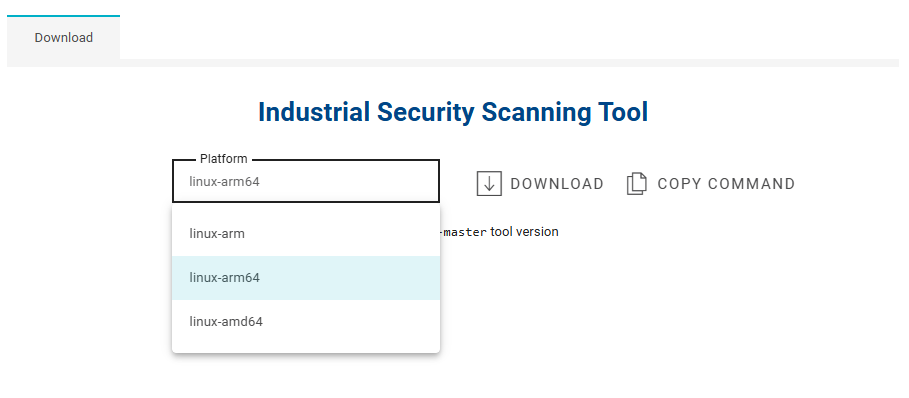
\includegraphics[width=1.0\textwidth]{chapters/05/assets/cloud-app-frontend}
  \caption{Cloud app frontend}
  \label{fig:cloud-app-frontend}
\end{figure}

The endpoint is a public REST API that is implemented by a controller on the cloud app backend. The controller is responsible for handling the incoming requests from the frontend and for forwarding them to the respective methods. The controller is also responsible for handling the authentication with the platform. The controller asks the related service model to actually list the available architectures and returns the final download link.

The endpoint is available at the \texttt{/v1/cli-release} base path; in particular, the \texttt{/platforms} path returns a dynamic list of the available architectures at that time, and the \texttt{/:version/:platform} path returns the actual download link for the specific version and platform. The download link is a direct link to the storage bucket that contains the binaries.

Notice that, although the app is accessible using a private account but the download link is public, we do not consider this a security issue because of the initial stage of the project and the limited access to the preview version of the app. In fact, only the company testers can access it at this time. Future work will be to implement a proper authentication system to access the download link.

\subsection{Support internationalization}

The support for different languages is a fundamental step for a company with a global presence. The company is interested in the possibility to offer the tool in different languages, in order to make it more accessible to customers.

In order to support internationalization, also known as \textit{i18n} because of the 18 letters between the \textit{i} and the \textit{n}, we use the \texttt{vue-i18n} package to translate the cloud app. The package is a plugin for VueJS that provides the i18n features to the application and it is available on the public NPM registry. The package allows to define the translations in a JSON file and to use them in the application by using the \texttt{\$t} function. The package also provides the ability to switch the language at runtime.

Also the tool is translated into different languages, primarily in English and Italian. The translations are again stored in different YAML files, one for each language, and they are loaded at runtime by the tool. The tool uses the \texttt{go-i18n} package. We did some wrapper functions to make the package similar to the way it works in the application by exposing a \texttt{t} function used to return the translation of a key. We decided to use a YAML translation file because it is even easier to read and write than a JSON file.

Both the translation methods support the variable replacement, that is the ability to replace a placeholder in the translation with a value. This is useful for example to translate a sentence that contains a variable part, like a number or a name. Also, they support pluralization, that is the ability to translate a sentence in different ways depending on the number of items. A clear example is the translation of the word \textit{item} in English, which is translated in two different ways depending on the number of items: \textit{item} for one item and \textit{items} for zero or more than one item. The pluralization is done by using the \texttt{one}, \texttt{other} and \texttt{few} keys in the translation file. The \texttt{one} key is used for the singular form, the \texttt{other} key is used for the plural form, and the \texttt{few} key is used for the few form. The package automatically selects the correct form based on the number of items passed as parameter.

Usually, the names of these functions are very short to reduce the verbosity in the code, given that they are used really really often in the code.

\section{Second sprint retrospective}

With this last task done, the second sprint has been completed successfully. All the expected modules have been implemented. The implementation of the modules has been straightforward. Compared to the first sprint, we adjusted the estimation of the complexity and the time needed to develop the new features and we have been able to complete the sprint in time. This is the end of the internship period. The company is satisfied by our job and it looks forward to further development.

